\documentclass[aspectratio=169,11pt]{beamer}

% ---------------------------------------------------------------------------
% Clean, neutral theme built from beamer primitives (no external theme pkgs
% needed, so this compiles on any plain TeX Live / MiKTeX install).
% ---------------------------------------------------------------------------
\usetheme{default}
\usefonttheme{professionalfonts}
\usepackage{lmodern}
\usepackage[T1]{fontenc}
\usepackage{booktabs}
\usepackage{graphicx}
\usepackage{array}
\usepackage{xcolor}

\definecolor{ink}{RGB}{35,35,35}
\definecolor{accent}{RGB}{31,78,121}
\definecolor{subtle}{RGB}{130,130,130}
\definecolor{amber}{RGB}{163,110,20}

\setbeamercolor{normal text}{fg=ink,bg=white}
\setbeamercolor{title}{fg=ink,bg=white}
\setbeamercolor{frametitle}{fg=accent,bg=white}
\setbeamercolor{structure}{fg=accent}
\setbeamercolor{block title}{fg=white,bg=accent}
\setbeamercolor{block body}{fg=ink,bg=accent!8}
\setbeamercolor{block title alerted}{fg=white,bg=amber}
\setbeamercolor{block body alerted}{fg=ink,bg=amber!10}
\setbeamercolor{alerted text}{fg=amber}
\setbeamercolor{footline}{fg=subtle,bg=white}
\setbeamercolor{page number in head/foot}{fg=subtle,bg=white}

\setbeamertemplate{navigation symbols}{}
\setbeamertemplate{itemize items}[circle]
\setbeamertemplate{itemize subitem}[circle]
\setbeamerfont{frametitle}{series=\bfseries,size=\large}
\setbeamerfont{footline}{size=\scriptsize}

\setbeamertemplate{frametitle}{
  \nointerlineskip
  \begin{beamercolorbox}[wd=\paperwidth,leftskip=0.6cm,rightskip=0.6cm,ht=3.6ex,dp=1.2ex]{frametitle}
    \usebeamerfont{frametitle}\insertframetitle
  \end{beamercolorbox}
  {\color{accent}\rule{\paperwidth}{0.6pt}}
}

\setbeamertemplate{footline}{
  \leavevmode
  \hbox{\begin{beamercolorbox}[wd=\paperwidth,ht=2.4ex,dp=1.2ex,leftskip=0.6cm,rightskip=0.6cm]{footline}
    \usebeamerfont{footline}\insertshorttitle \hfill \insertframenumber{} / \inserttotalframenumber
  \end{beamercolorbox}}
}

% ---------------------------------------------------------------------------
% Metadata -- fill in before presenting
% ---------------------------------------------------------------------------
\title{Regulatory Data Infrastructure for EPA Clean Air Act Enforcement}
\subtitle{\texttt{caa-regdata}: a reproducible facility $\times$ year pipeline}
\author{[Your Name]}
\institute{[Lab / Program Name] \\ 10-Week Internship, Final Presentation}
\date{[Presentation Date]}

\begin{document}

\begin{frame}[plain]
  \titlepage
\end{frame}

% =============================================================================
\begin{frame}{Roadmap}
  \begin{enumerate}
    \item The problem and the mandate
    \item What I built: pipeline, datasets, panels
    \item A methods choice worth walking through
    \item Key findings
    \item Transition and handoff
    \item What I learned
  \end{enumerate}
  \vfill
  \small\color{subtle} 15 minutes presenting, 5 minutes questions.
\end{frame}

% =============================================================================
\section{Motivation}
\begin{frame}{The gap}
  \begin{itemize}
    \item Empirical work on Clean Air Act enforcement and compliance needs a \textbf{facility $\times$ year
      panel}: inspections, violations, enforcement actions, permits, emissions.
    \item EPA doesn't ship one.
    \begin{itemize}
      \item ICIS-Air (EPA ECHO) is a \textbf{live current snapshot} — no history.
      \item \textbf{Pre-2015 operating status} doesn't exist anywhere in the current extract at all.
    \end{itemize}
    \item Cooperative federalism (states enforce, EPA sets standards/backstops) means the relevant data is
      scattered across current and legacy systems that don't share identifiers.
  \end{itemize}
  \begin{block}{The mandate}
    Build the panel infrastructure — reproducibly, and documented well enough that someone returning to
    this cold in six months (or a coauthor who's never seen it) can pick it up.
  \end{block}
\end{frame}

% =============================================================================
\section{What I built}
\begin{frame}{Pipeline shape}
  \begin{center}
  \textbf{raw} (immutable) $\;\rightarrow\;$ \textbf{clean} (lossless, one asset/source) $\;\rightarrow\;$
  \textbf{8 datasets} (full universe) $\;\rightarrow\;$ \textbf{2 panels} (sample-restricted) $\;\rightarrow\;$
  \textbf{docs site}
  \end{center}
  \vspace{0.5em}
  \begin{itemize}
    \item \textbf{Sources:} ICIS-Air (current + 10 Wayback snapshots), AFS legacy, FRS coordinates, Census
      counties, combined emissions — all public, no DUA restrictions.
    \item \textbf{Cleaning:} every raw table gets one clean asset, every row and column kept — sample
      selection happens downstream, not here.
    \item One command rebuilds everything from raw: \texttt{Rscript code/RUN\_ALL.R}.
  \end{itemize}
\end{frame}

\begin{frame}{Design principles}
  \begin{itemize}
    \item \textbf{Raw is immutable} — nothing in \texttt{data/raw/} is ever hand-edited.
    \item \textbf{\texttt{renv}-pinned} — exact package versions, one \texttt{renv::restore()} away.
    \item \textbf{Provenance logged} — every raw file's source URL, fetch date, and checksum in
      \texttt{MANIFEST.csv}.
    \item \textbf{Tests as invariants} — not correctness-by-eyeball; asserted in \texttt{tests/} and at
      build time (e.g.\ event totals must sum, no \texttt{\_DUP} column may exceed its parent).
    \item \textbf{Every construction choice logged as I made it} — not reconstructed after the fact — in
      \texttt{*\_construction\_decisions.md} briefs: the decision, the alternative not taken, and why.
  \end{itemize}
\end{frame}

\begin{frame}{The Wayback reconstruction}
  \begin{itemize}
    \item EPA's current ICIS-Air extract retains \textbf{no operating-status history} — a facility's status
      today is all you get.
    \item I pulled \textbf{10 annual snapshots} (2015--2017, 2019--2025) of the ICIS-Air bulk download from
      the Internet Archive Wayback Machine, each pinned to a capture confirmed byte-for-byte against the
      previously staged files.
    \item Reconstructs, year by year: operating status, facility entry/exit, program-active flags — none of
      which EPA itself retains for the pre-2015 window at all.
    \item Coverage: \textbf{42.1\%} of the full 21-year rectangle; \textbf{$\sim$80\%} of facility-years
      within Wayback's own 2015--2025 window.
  \end{itemize}
\end{frame}

\begin{frame}{Eight deliverable datasets}
  \footnotesize
  \begin{tabular}{@{}l l l@{}}
    \toprule
    \textbf{Dataset} & \textbf{Grain} & \textbf{Contents} \\
    \midrule
    \texttt{regulatory} & facility $\times$ year & ICIS event counts + facility characteristics \\
    \texttt{operating} & facility $\times$ year & Wayback status, program-active flags, entry/exit \\
    \texttt{wayback\_only\_facilities} & facility $\times$ year & facilities Wayback saw that ICIS no longer lists \\
    \texttt{hpv\_spells} & spell & one row per High-Priority-Violation spell \\
    \texttt{hpv\_active} & facility $\times$ year & HPV-active flag, collapsed from spells \\
    \texttt{penalties} & formal action & penalties + multi-facility settlement key \\
    \texttt{coordinates} & facility & FRS lat/lon, county, geocode diagnostics \\
    \texttt{pipeline} & facility $\times$ year & linked evaluation $\to$ violation $\to$ enforcement \\
    \texttt{emissions} & facility $\times$ year & pollutant quantities (VOC/PM/NO$_x$/SO$_2$/HAP/GHG) \\
    \bottomrule
  \end{tabular}
  \vspace{0.6em}
  \small Built once over the \textbf{full facility universe} — any sample restriction is a downstream
  filter, not a pre-built panel.
\end{frame}

\begin{frame}{Two continuous panels}
  \begin{itemize}
    \item \textbf{\texttt{major\_synmin\_continuous\_2015\_2025}} — 20{,}261 facilities, 222{,}871
      facility-years.
    \item \textbf{\texttt{electric\_continuous\_2015\_2025}} — 1{,}913 facilities, 21{,}043 facility-years
      (a strict subset: every electric facility is also in major\_synmin).
    \item \textbf{Continuity screen:} \texttt{ACTIVE\_BROAD == 1} in every single year, 2015--2025 — no
      partial credit; one confirmed-inactive or no-evidence year fails the screen.
    \item Built directly from the datasets layer, not from raw processed assets — so every downstream fix
      to the eight datasets propagates automatically.
  \end{itemize}
\end{frame}

% =============================================================================
\section{Methods spotlight}
\begin{frame}{Methods spotlight: two incomplete signals}
  \textbf{Question the panel needs answered: was this facility real in year $Y$?}
  \begin{columns}[T]
    \column{0.48\textwidth}
    \textbf{\texttt{OPERATING}} (Wayback)
    \begin{itemize}
      \small
      \item Full 2015--2025 coverage
      \item \textbf{92{,}080 facilities} are Wayback-confirmed operating in some year with \textbf{zero}
        ICIS events, ever — mostly never-inspected minor sources
    \end{itemize}
    \column{0.48\textwidth}
    \textbf{\texttt{ICIS\_OBSERVED}} (events)
    \begin{itemize}
      \small
      \item Full 2005--2025 coverage
      \item Of 133{,}753 facilities with $\geq$1 in-window ICIS event, \textbf{15{,}699 (11.7\%)} — mostly
        active only pre-2015 — have \textbf{no} Wayback-confirmed operating year at all
    \end{itemize}
  \end{columns}
  \vspace{0.6em}
  \begin{alertblock}{Neither signal alone is sufficient}
    Each one misses facility-years the other one catches.
  \end{alertblock}
\end{frame}

\begin{frame}{Methods spotlight: \texttt{ACTIVE} / \texttt{ACTIVE\_BROAD}}
  \begin{block}{The fix}
    \texttt{ACTIVE} = \texttt{OPERATING==1} \textbf{OR} \texttt{ICIS\_OBSERVED==1}, evaluated
    \textbf{year by year}. \\
    \texttt{ACTIVE\_BROAD} additionally unions emissions/GHG reporting for that year.
  \end{block}
  \begin{itemize}
    \item Verified to nest monotonically end-to-end:
      $\texttt{OPERATING}{=}1 \Rightarrow \texttt{ACTIVE}{=}1 \Rightarrow \texttt{ACTIVE\_BROAD}{=}1$ —
      checked row by row, 0 violations.
    \item \textbf{Why year-varying, not a facility-level ``ever'' flag:} a facility real in 2008 isn't
      necessarily real in 2022. Collapsing to ``ever'' is a trivial \texttt{any()} a downstream user can do
      themselves; recovering per-year detail from an ``ever'' flag is impossible.
    \item This \emph{is} the continuity screen behind both panels.
  \end{itemize}
\end{frame}

% =============================================================================
\section{Findings}
\begin{frame}{Findings I: what's actually observed}
  \begin{itemize}
    \item Only \textbf{12.6\%} of the full regulatory rectangle (279{,}665 facilities $\times$ 21 years) is
      observed at all — \textbf{52.2\%} of facilities have zero in-window ICIS events.
    \item Coverage is \textbf{not} a random sample: EPA's own Minimum Data Requirements exempt most ordinary
      minor sources from reporting unless a specific trigger fires. Facility-year coverage is endogenous to
      size/class.
  \end{itemize}
  \begin{center}
    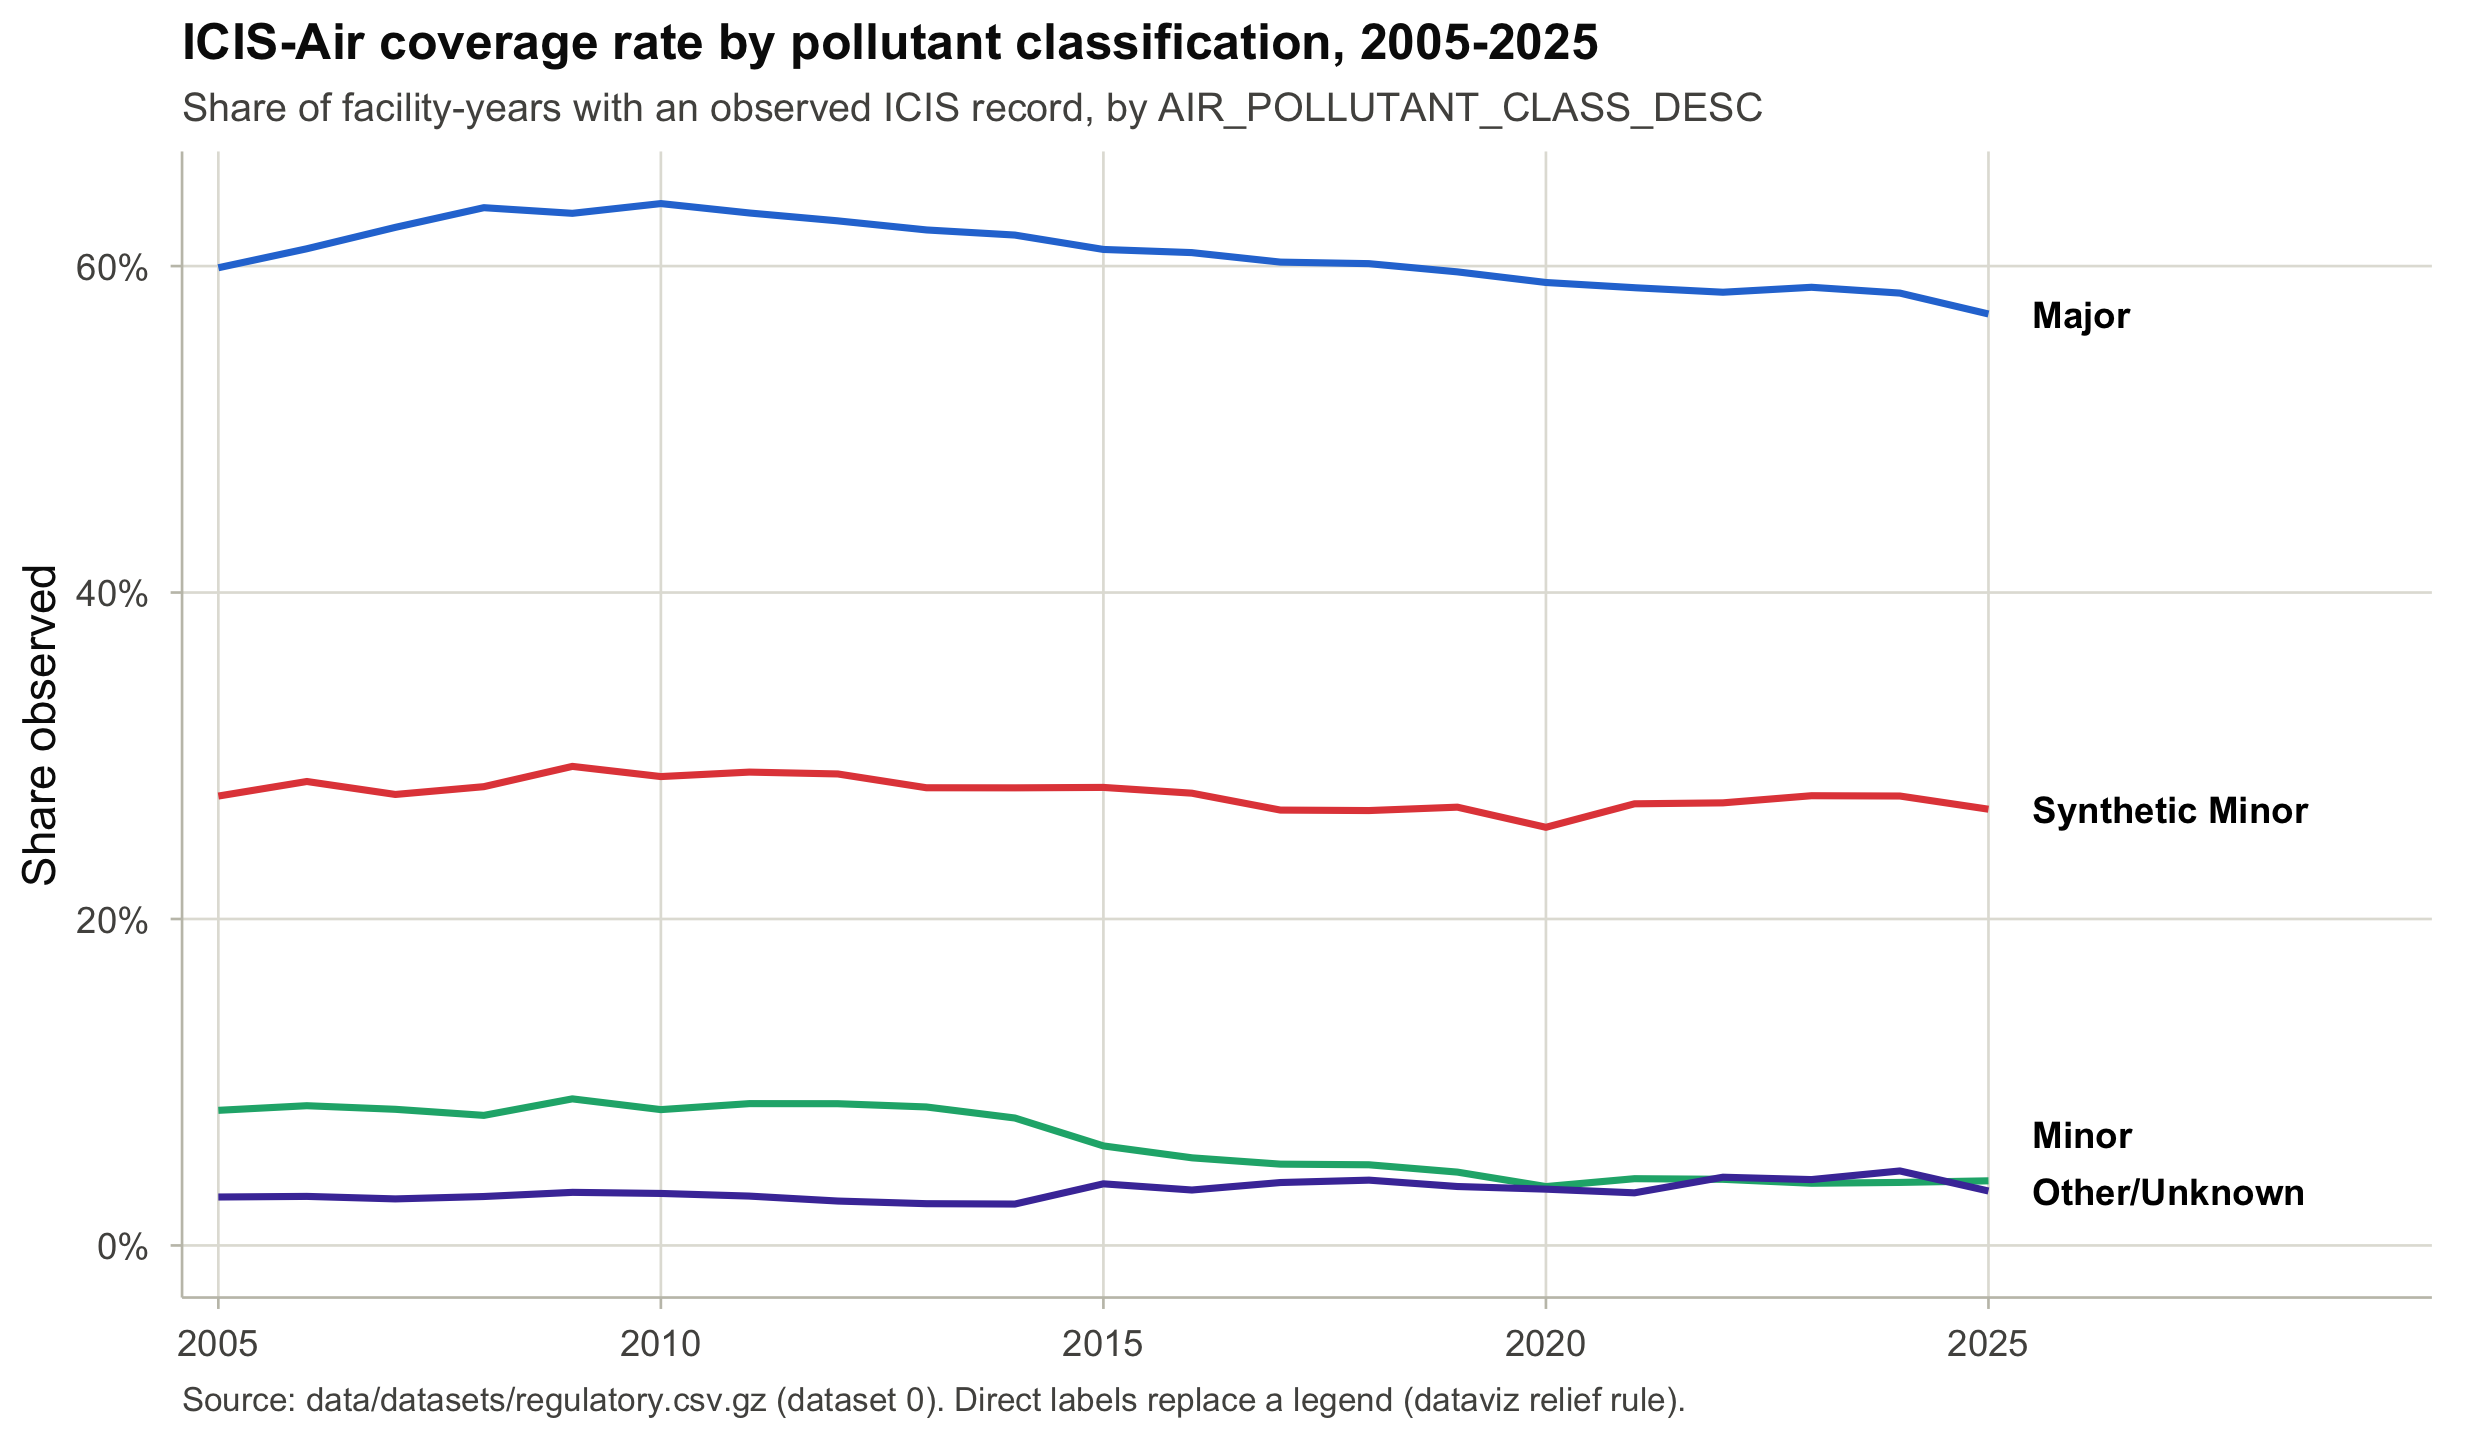
\includegraphics[width=0.72\textwidth]{../output/figures/datasets/regulatory/reg_coverage_by_classification_over_time.png}
  \end{center}
\end{frame}

\begin{frame}{Findings II: bugs I found and fixed}
  \begin{itemize}
    \item \textbf{\texttt{EMITS\_HAP} false negatives:} matched only the literal phrase
      ``HAZARDOUS AIR POLLUTANT,'' missing most HAPs recorded under a chemical name. Fixed with a CAS-number
      join against the official \S112(b) list (188 substances) — corrected count: \textbf{67{,}011}
      facilities (24.0\%).
    \item \textbf{\texttt{N\_VIOL\_NSPS} scope creep:} a substring match accidentally pulled in 418 rows
      belonging to a related-but-distinct program code.
    \item \textbf{\texttt{N\_PENALTY\_ACTION} undercount:} an exact-text match missed four expedited
      settlement variants of the same action — a \textbf{2.9\%} undercount of the true family, fixed by
      matching the code prefix instead of the description text.
  \end{itemize}
\end{frame}

\begin{frame}{Findings III: duplicate load isn't uniform}
  \begin{itemize}
    \item \textbf{Informal} enforcement rows: $\sim$\textbf{48\%} are event-key duplicates.
    \item \textbf{Formal} enforcement rows: $\sim$\textbf{1\%}.
    \item A raw row count overstates informal activity roughly 2$\times$ relative to formal — not disclosed
      unless you check.
    \item \textbf{Multi-facility settlements} repeat the same penalty figure across every co-defendant's
      row. Summing \texttt{PENALTY\_AMOUNT} across facilities double- (or multiply-) counts that
      settlement: \textbf{4.6\%} of total penalty dollars in the broader panel, up to \textbf{11.6\%} in the
      electric panel.
    \item Every count and dollar figure in the datasets layer carries its own \texttt{\_DUP} column rather
      than silently deduping — the choice is left to the analyst, not made for them.
  \end{itemize}
\end{frame}

\begin{frame}{Findings IV: descriptive patterns in the panels}
  \small\color{subtle}\emph{Descriptive, not causal — no design here licenses a claim about \textit{why}.}
  \normalsize\color{ink}
  \begin{itemize}
    \item \textbf{HPV-active share roughly halved, 2015 $\to$ 2025}, in both panels (major\_synmin:
      4.54\%$\to$2.31\%; electric: 5.02\%$\to$1.99\%).
    \item \textbf{Electric utilities are inspected more but flagged less}: higher mean inspections (2.49 vs.\
      1.85) but lower mean violations (0.13 vs.\ 0.17) and enforcement (0.26 vs.\ 0.42) per observed
      facility-year than the broader major/synmin population — more scrutiny, proportionally fewer
      findings.
  \end{itemize}
  \begin{center}
    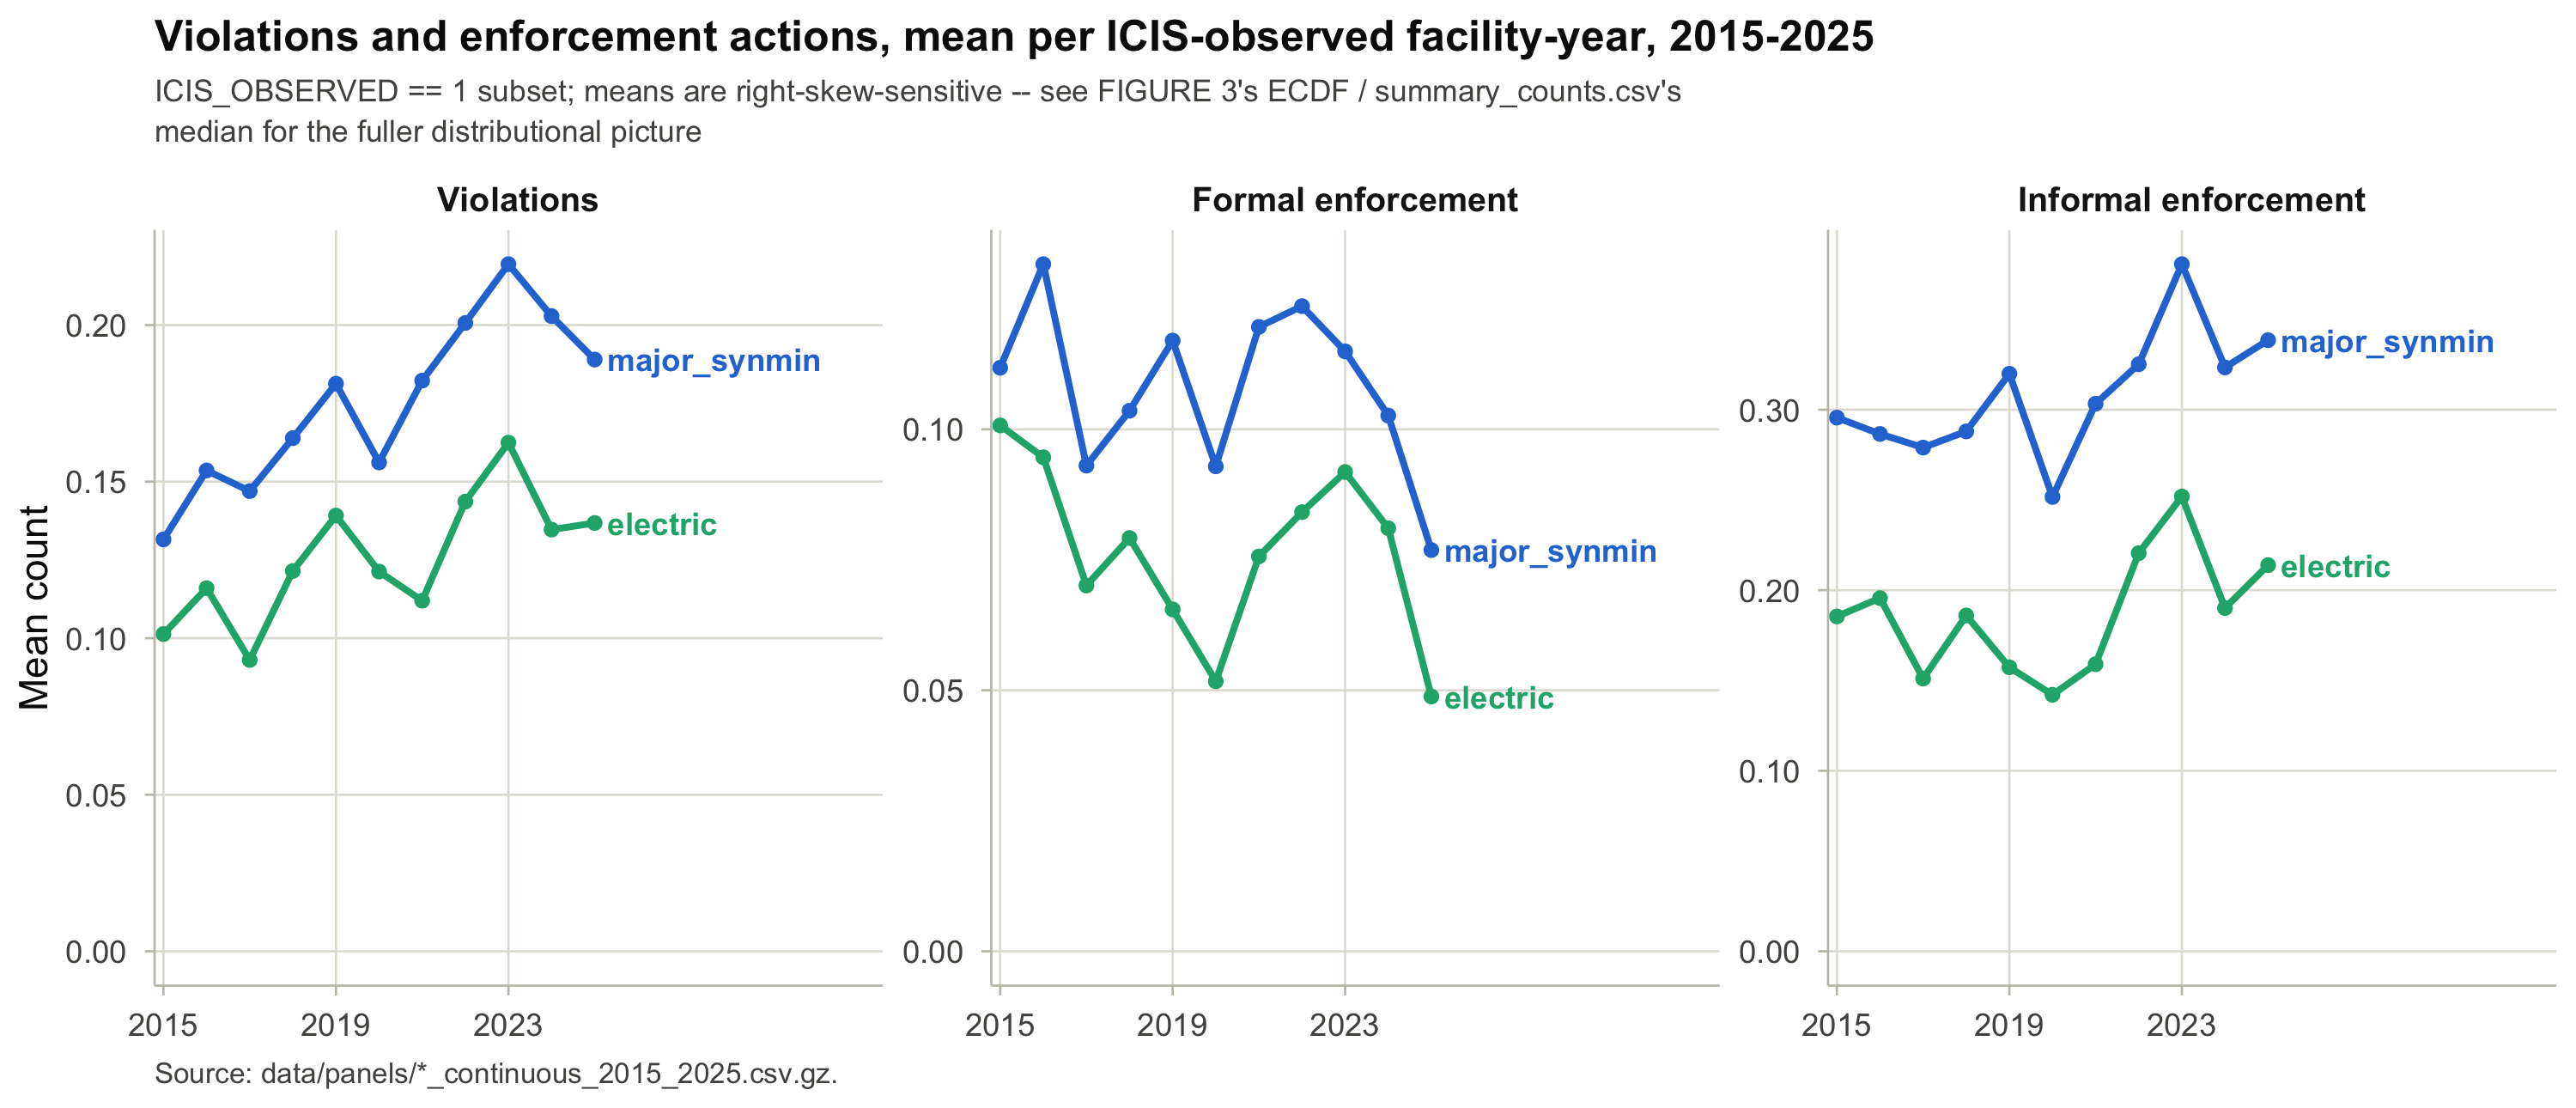
\includegraphics[width=0.62\textwidth]{../output/figures/panels/panel_violations_enforcement.png}
  \end{center}
\end{frame}

\begin{frame}{Findings IV, continued: penalties}
  \begin{itemize}
    \item Right-skewed in both panels, as expected — most cases settle small, a few drive the mean.
    \item major\_synmin: median \$9{,}800, p95 \$298{,}196, max \$43.1M.
    \item electric: median \$8{,}000 (close), but max only \$4.9M — the largest settlements concentrate
      \emph{outside} electric generating units specifically.
    \item \small\color{subtle} Totals are naive — not corrected for the duplicate-settlement broadcast in
      Findings III. Don't cite \$1.16B / \$58.3M as corrected figures.
  \end{itemize}
  \begin{center}
    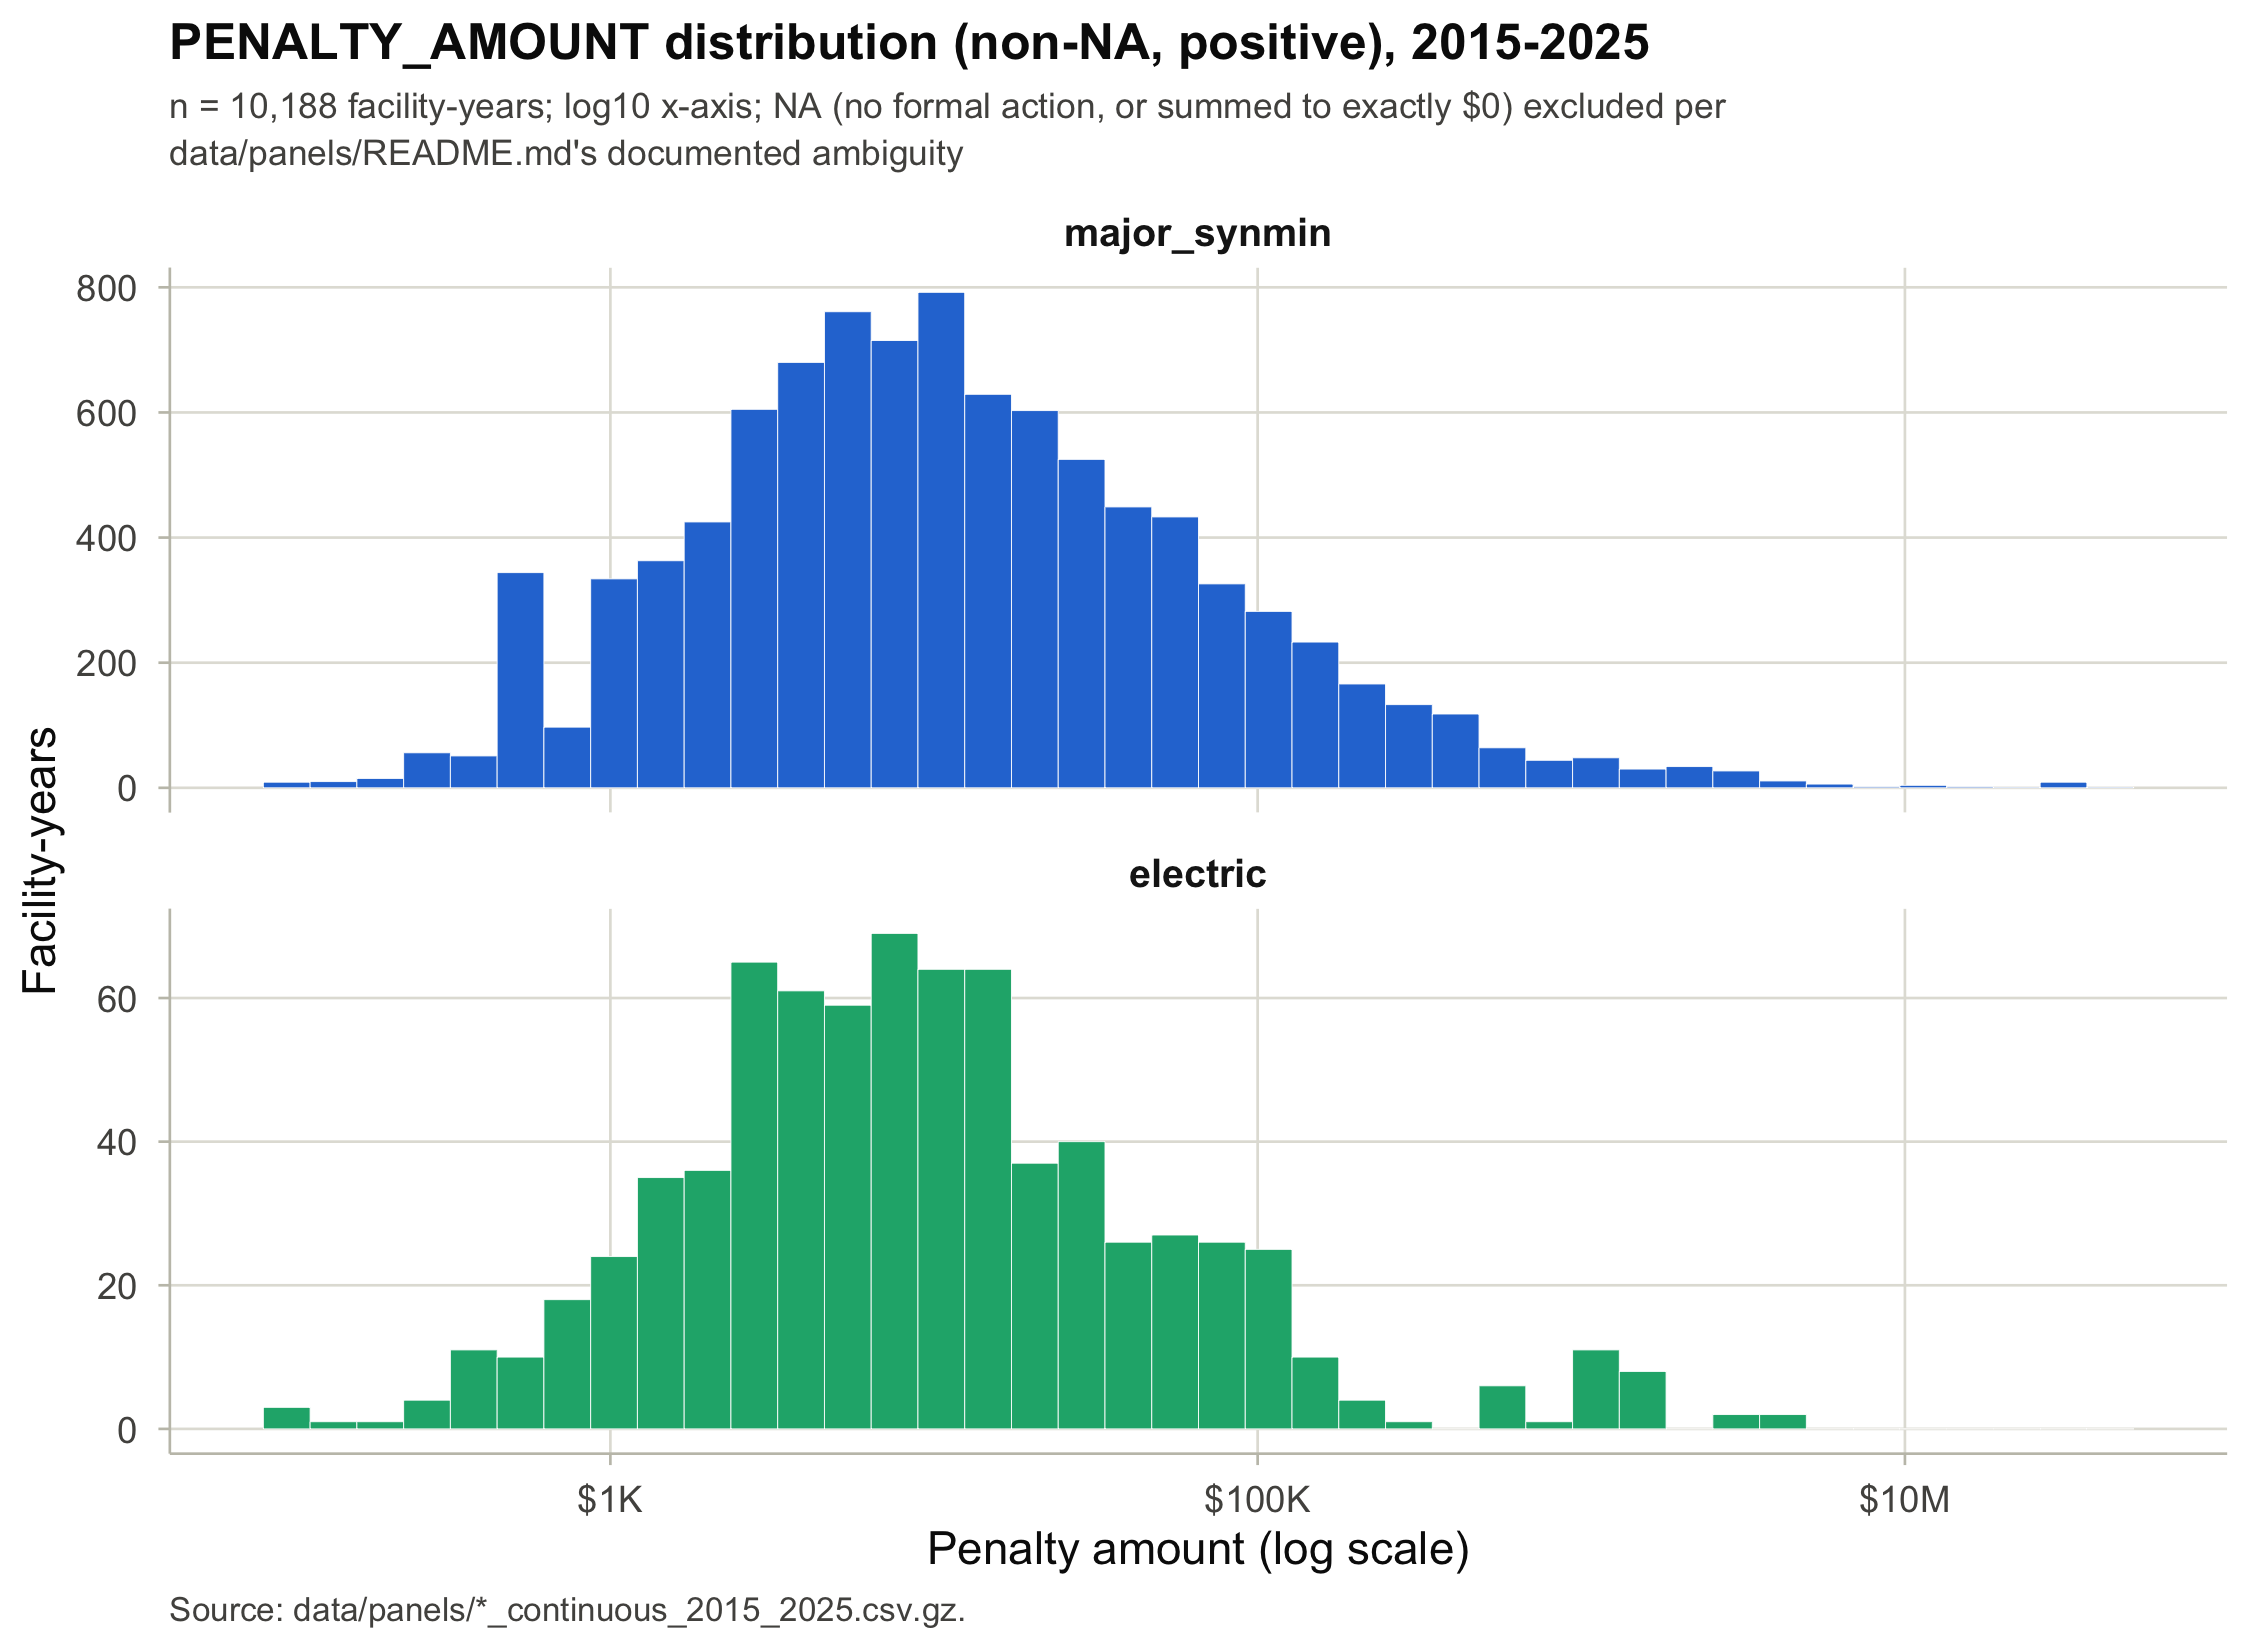
\includegraphics[width=0.58\textwidth]{../output/figures/panels/panel_penalty_dist.png}
  \end{center}
\end{frame}

% =============================================================================
\section{Handoff}
\begin{frame}{Transition and handoff: done}
  \begin{itemize}
    \item All \textbf{8 datasets} built and audited over the full facility universe.
    \item Both \textbf{continuous panels} built, profiled, and cross-checked (e.g.\ electric confirmed as a
      strict subset of major\_synmin, every run).
    \item \textbf{Docs site} (4-page static site) generated from the data — can't drift from it.
    \item \textbf{Tests} passing; every construction decision logged in the \texttt{briefs/} — not just
      what was built, but the alternative rejected and why.
  \end{itemize}
\end{frame}

\begin{frame}{Transition and handoff: open}
  \begin{itemize}
    \item \textbf{AFS$\leftrightarrow$ICIS crosswalk} (a candidate pre-2015 operating-status signal from the
      legacy system): investigated this session, \textbf{explicitly left unresolved}. The
      facility-identifier bridge (via FRS) only matches \textbf{59.3\%} of AFS records on its best rule —
      not clearly ``good enough'' to build on.
    \item \textbf{\texttt{PENALTY\_AMOUNT}'s NA-vs-exactly-\$0 ambiguity} is unresolved — currently
      indistinguishable from ``no formal action at all.''
    \item \textbf{License:} TBD — needs a decision before any publication or redistribution.
    \item \textbf{2025 as a data point:} likely reporting lag, not a real activity drop — re-check on a
      later refresh before treating it as a trend endpoint.
  \end{itemize}
  \vspace{0.4em}
  \textbf{Start here:} \texttt{README.md} $\to$ \texttt{code/README.md} $\to$ the
  \texttt{*\_construction\_decisions.md} briefs.
\end{frame}

% =============================================================================
\section{Lessons}
\begin{frame}{What I learned}
  \begin{itemize}
    \item \textbf{Reproducible pipeline design at production scale} — \texttt{renv} pinning, provenance
      manifests, tests as invariants rather than eyeballed checks.
    \item \textbf{CAA regulatory institutional knowledge} — SIP/NSPS/NESHAP-MACT/Title V/PSD-NNSR, and the
      enforcement pipeline from compliance evaluation through violation, informal/formal action, and
      penalty.
    \item \textbf{Historical reconstruction from web archives} — pulling and validating Wayback Machine
      snapshots to recover history the live source doesn't retain.
    \item \textbf{Decision-logging as a research practice}, not just code hygiene — writing the ``why not
      X'' next to the ``what,'' so re-entry doesn't require re-deriving it.
    \item \textbf{Descriptive vs.\ causal discipline} — separating ``the data show $X$'' from ``$X$ is
      caused by $Y$,'' and saying so explicitly on the slide, not just in a footnote.
  \end{itemize}
\end{frame}

\begin{frame}[plain]
  \begin{center}
    {\Large\bfseries Thank you}\\[0.5em]
    Questions?
  \end{center}
\end{frame}

% =============================================================================
% Backup slides
% =============================================================================
\appendix
\begin{frame}{Backup: the AFS$\leftrightarrow$ICIS crosswalk in detail}
  \begin{itemize}
    \item AFS (legacy, frozen 2014) uses \texttt{AFS\_ID}; ICIS-Air (this repo's spine) uses
      \texttt{PGM\_SYS\_ID} — no shared format.
    \item Two-hop bridge via FRS: \texttt{AFS\_ID} $\to$ \texttt{REGISTRY\_ID}
      (\texttt{FRS\_PROGRAM\_LINKS.csv}) $\to$ \texttt{PGM\_SYS\_ID} (\texttt{ICIS-AIR\_FACILITIES.csv}).
    \item Hop 1 (AFS $\to$ FRS): best rule matches \textbf{59.3\%} of AIR-tagged FRS rows to a real
      \texttt{AFS\_ID}.
    \item Hop 2 (FRS $\to$ ICIS): clean, nearly unambiguous — only 0.13\% of hop-1-linked IDs map to more
      than one facility.
    \item Reproduced the predecessor project's baseline exactly before trusting any new number.
    \item Open question, not a rejected idea: is 59.3\% coverage ``good enough'' to build a pre-2015
      operating proxy on? Left for whoever picks this up next.
  \end{itemize}
\end{frame}

\begin{frame}{Backup: the zero-vs-NA discipline}
  \begin{itemize}
    \item A facility-year is \texttt{ICIS\_OBSERVED == 1} iff ICIS holds $\geq$1 row across any of the six
      event assets that year.
    \item \textbf{Observed:} a count of 0 for some other measure is a true zero.
    \item \textbf{Not observed:} every count is \texttt{NA} — unknown, not zero.
    \item Applied uniformly across the datasets layer; verified at build time (observed rows never
      \texttt{NA}, unobserved rows always \texttt{NA}, across all 48 event-count columns).
    \item Why it matters: coding absence as 0 would silently assert ``confirmed zero activity'' for
      facility-years that were simply never looked at.
  \end{itemize}
\end{frame}

\end{document}
